\subsection{Brugergr�nseflade}
Der er blevet udformet en skitse over brugergr�nsefladen p� brugersystemet, s� det er muligt at f� en id� om, hvordan det grafiske vil komme til at se ud. Det er vigtigt at understrege, at det er en \underline{skitse}, og at den endelige brugergr�nseflade ikke n�dvendigvis vil ligne denne fuldst�ndigt:\\

\begin{figure}[h]
\centering
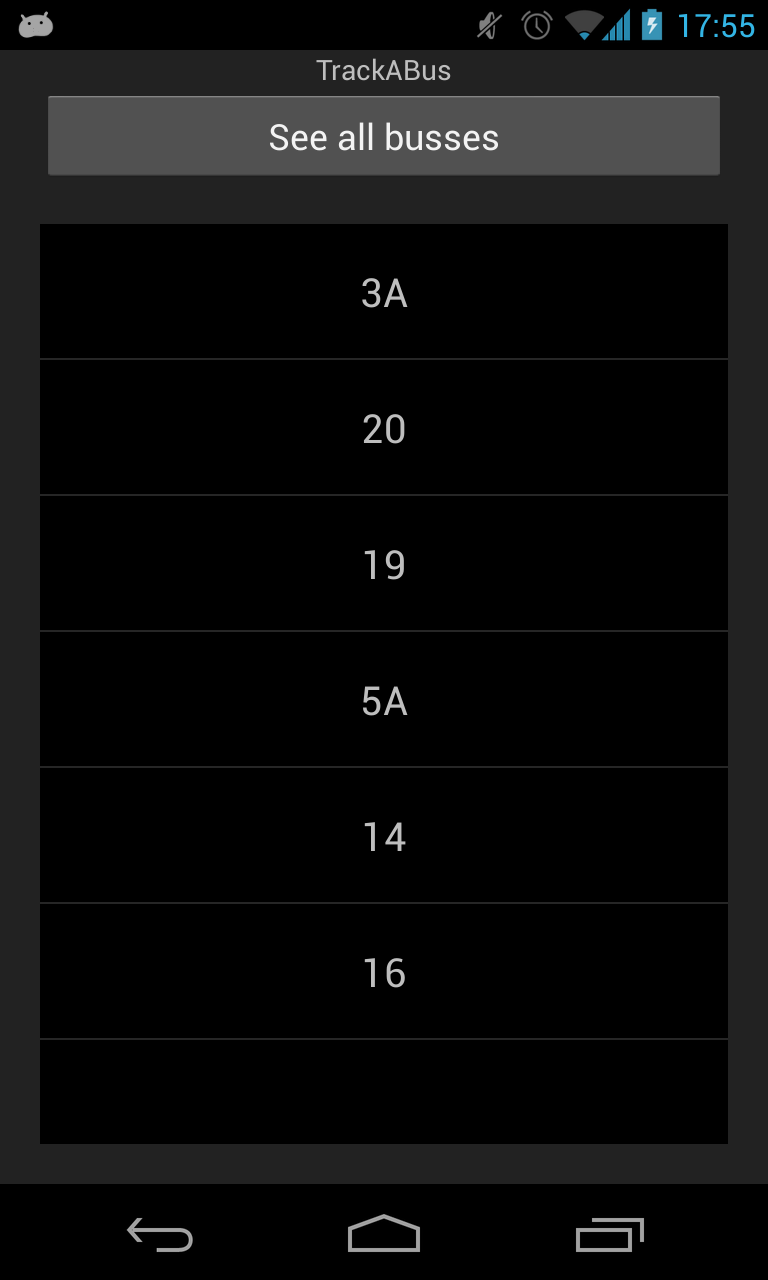
\includegraphics[scale=0.2]{Eksterne_grEnseflader/GUI/MainScreen.png}
\caption{Startsk�rm\\ Dette viser en grov skitse af hvordan startsk�rmen p� brygersystemet ser ud, her er det muligt at tilg� listen over alle busruter(�verst) samt se listen af busruter der er blevet favoriseret(nederst).}
\end{figure}

\begin{figure}[h]
\centering
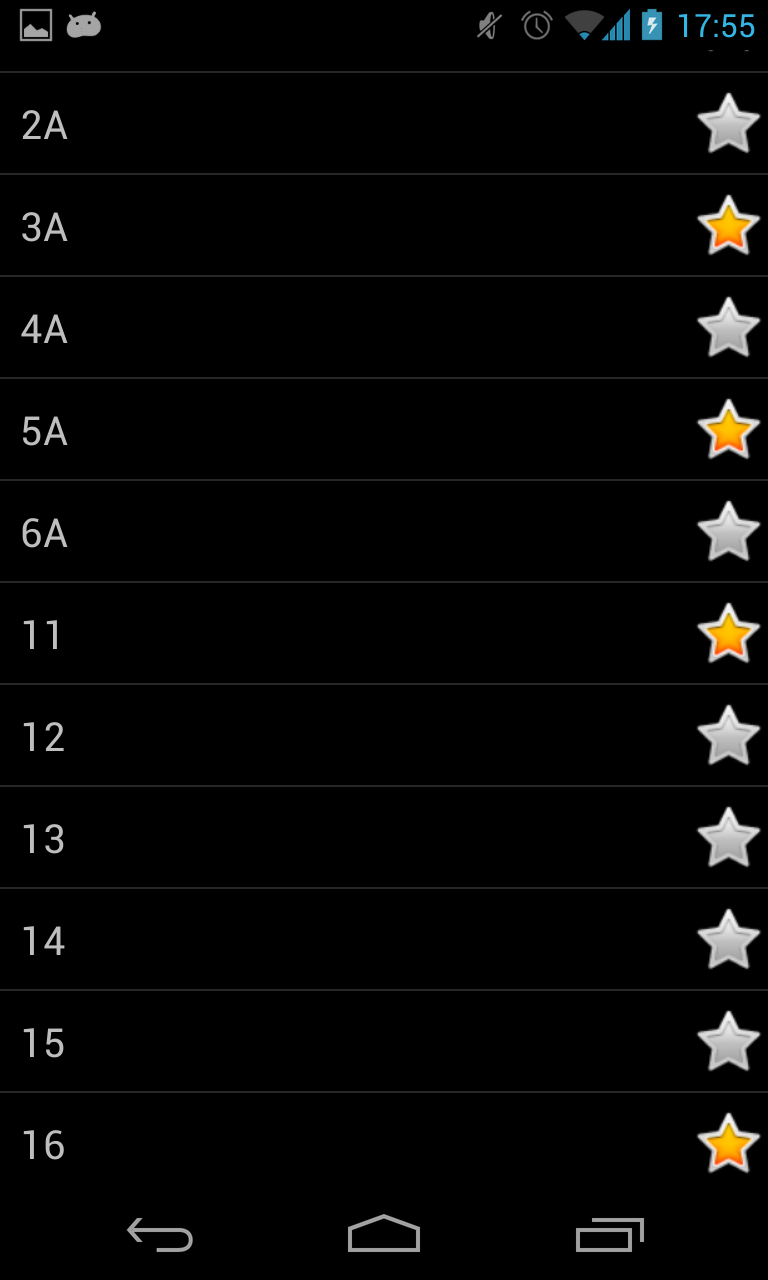
\includegraphics[scale=0.2]{Eksterne_grEnseflader/GUI/RouteList.png}
\caption{Busrute listen\\ Dette viser en grov skitse over listen af busruter der kan v�lges i brugersystemet, her er det muligt at favoriser forskellilge ruter. }
\end{figure}

\begin{figure}[u]
\centering
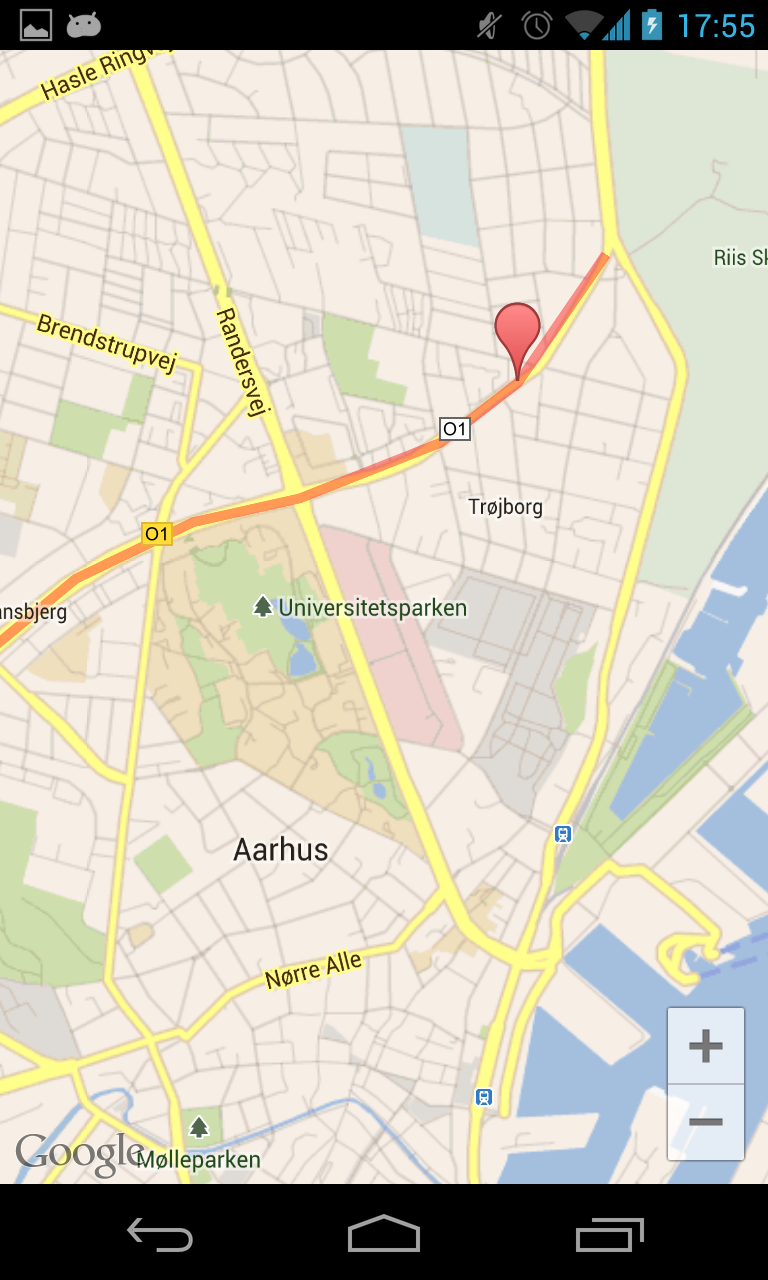
\includegraphics[scale=0.2]{Eksterne_grEnseflader/GUI/Map.png}
\caption{Map\\ Dette viser en grov skitse af det map, hvorp� busruten, stoppesteder og bussen vil blive indtegnet}
\end{figure}